% Concept trial only. Do not \input this from the paper until the user keeps the figure.
% No existing label was found. fig:limit-demand-trial is a proposed name, not an old label.
% VLDB sigconf figure* width: 178mm (textwidth about 506.3pt). Do not scale this into one column.
\begin{figure*}[t]
  \centering
  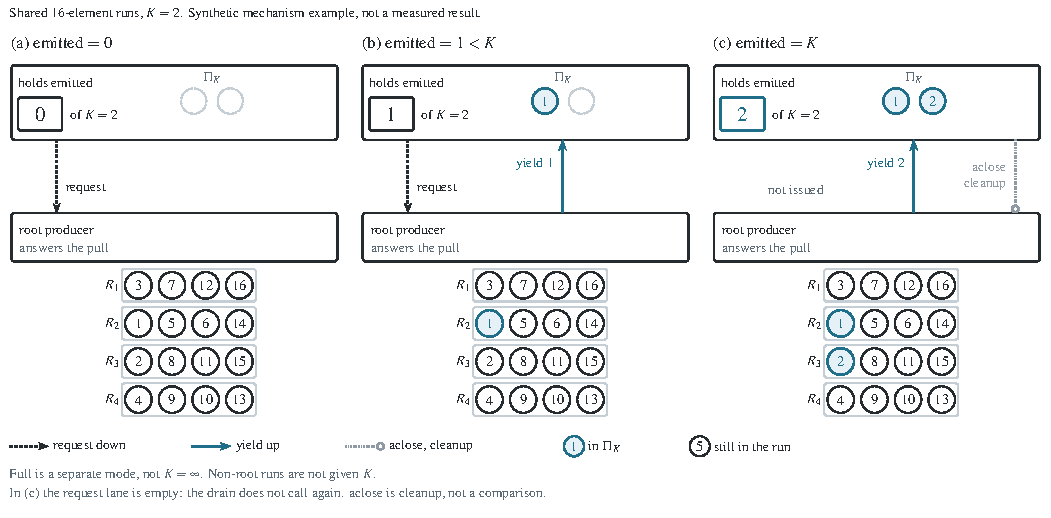
\includegraphics[width=\textwidth]{limit-ondemand.pdf}
  \caption{Concept trial of demand-driven LIMIT on the shared 16-element runs, $K{=}2$.
  Not a measured result and not an execution trace.
  The downstream drain holds \emph{emitted}.
  A dashed arrow is one request downward; a solid arrow is one yield upward.
  In (c), \emph{emitted}${=}K$, so the next request is not issued, and the hollow items stay in the runs.
  The gray dotted arrow is \texttt{finally} \texttt{aclose}, drawn as cleanup.
  Full is a separate execution mode, not $K{=}\infty$.
  Keep this figure only if this reading is wanted.}
  \label{fig:limit-demand-trial}
\end{figure*}
